\documentclass[12pt,a4paper,english]{article}
\usepackage{graphicx}
\usepackage[english]{babel}
\usepackage[utf8]{inputenc}
%\usepackage{listings}
\usepackage{multirow}
\usepackage{epstopdf}
\usepackage{amsmath}
\usepackage{amssymb}
\usepackage{mathpazo}
\usepackage{csquotes}
\usepackage{siunitx}
\usepackage{tikz}
\usepackage{booktabs}
\graphicspath{{./fig/}}

\setlength{\hoffset}{-1in} \setlength{\textwidth}{18cm}
\setlength{\oddsidemargin}{1.5cm}
\setlength{\evensidemargin}{1.5cm}
\setlength{\marginparsep}{0.7em}
\setlength{\marginparwidth}{0.5cm}

\setlength{\voffset}{-1.9in}
\setlength{\headheight}{12pt}
\setlength{\topmargin}{2.6cm}
   \addtolength{\topmargin}{-\headheight}
\setlength{\headsep}{3.5cm}
   \addtolength{\headsep}{-\topmargin}
   \addtolength{\headsep}{-\headheight}
\setlength{\textheight}{27cm}

%% How should floats be treated?
\setlength{\floatsep}{12 pt plus 0 pt minus 8 pt}
\setlength{\textfloatsep}{12 pt plus 0pt minus 8 pt}
\setlength{\intextsep}{12 pt plus 0pt minus 8 pt}

\tolerance2000
\emergencystretch20pt

%% Text appearence
% English text
\newcommand{\eg}[1]%
  {\selectlanguage{english}\textit{#1}\selectlanguage{austrian}}

\newcommand{\filename}[1]
  {\begin{small}\texttt{#1}\end{small}}

\newcommand\IFT{\unitlength1mm\begin{picture}(10,2) \put (1,1)
{\circle{1.7}} \put(2,1){\line(1,0){5}} \put(8,1)
{\circle*{1.7}}\end{picture}}
\newcommand\FT{\unitlength1mm\begin{picture}(10,2) \put (1,1)
{\circle*{1.7}} \put(2,1){\line(1,0){5}} \put(8,1)
{\circle{1.7}}\end{picture}}

% A box for multiple choice problems
\newcommand{\choicebox}{\fbox{\rule{0pt}{0.5ex}\rule{0.5ex}{0pt}}}

\newenvironment{truefalse}%
  {\bigskip\par\noindent\makebox[1cm][c]{true}\hspace{3mm}\makebox[1cm][c]{false}
   \begin{list}%
   {\makebox[1cm][c]{\choicebox}\hspace{3mm}\makebox[1cm][c]{\choicebox}}%
   {\setlength{\labelwidth}{2.31 cm}\setlength{\labelsep}{3mm}
    \setlength{\leftmargin}{2.61 cm}\setlength{\listparindent}{0pt}
    \setlength{\itemindent}{0pt}}%
  }
  {\end{list}}

\newcounter{theexercise}\setcounter{theexercise}{1}
\newenvironment{exercise}[1]%
  {\bigskip\par\noindent\begin{nopagebreak}
   \textsf{\textbf{Exercise \arabic{theexercise}}}\quad
      \textsf{\textit{#1}}\\*[1ex]%
\stepcounter{theexercise}\hspace{2ex}\end{nopagebreak}}
  {\par\pagebreak[2]}

\renewcommand{\labelenumi}{\alph{enumi})}
\renewcommand{\labelenumii}{\arabic{enumii})}

% A box to tick for everything which has to done
\newcommand{\abgabe}{\marginpar{$\Box$}}
% Margin paragraphs on the left side
\reversemarginpar

% Language for listings
%\lstset{language=Vhdl,
%  basicstyle=\small\tt,
 % keywordstyle=\tt\bf,
 % commentstyle=\sl}

% No indention
\setlength{\parindent}{0.0cm}
% Don't number sections
\setcounter{secnumdepth}{0}

\DeclareMathOperator{\atantwo}{atan2}

%% Beginning of the text

\begin{document}
\selectlanguage{english}
\pagestyle{plain}

\thispagestyle{empty}
\noindent
\begin{minipage}[b][4cm]{1.0\textwidth}
    \begin{center}
        \begin{bf}
            \begin{large}
                Digital Signal Processing 2024S -- Assignment 2
            \end{large} \\
            \vspace{0.3cm}
            \begin{Large}
                Discrete Time Signals, Convolution, DTFT
            \end{Large} \\
            \vspace{0.3cm}
        \end{bf}
        \begin{large}
            Group 52\\
            Laurenz Weixlbaumer, k11804751\\
            Jannik Jungmann, k12103135\\
        \end{large}
    \end{center}
\end{minipage}

\noindent \rule[0.8em]{\textwidth}{0.12mm}\\[-0.5em]

\begin{exercise}{Discrete Time Signals}
    \begin{enumerate}
        \item See Figure \ref{fig:ex1_1}.
        \begin{figure}[hb]
            \centering    
            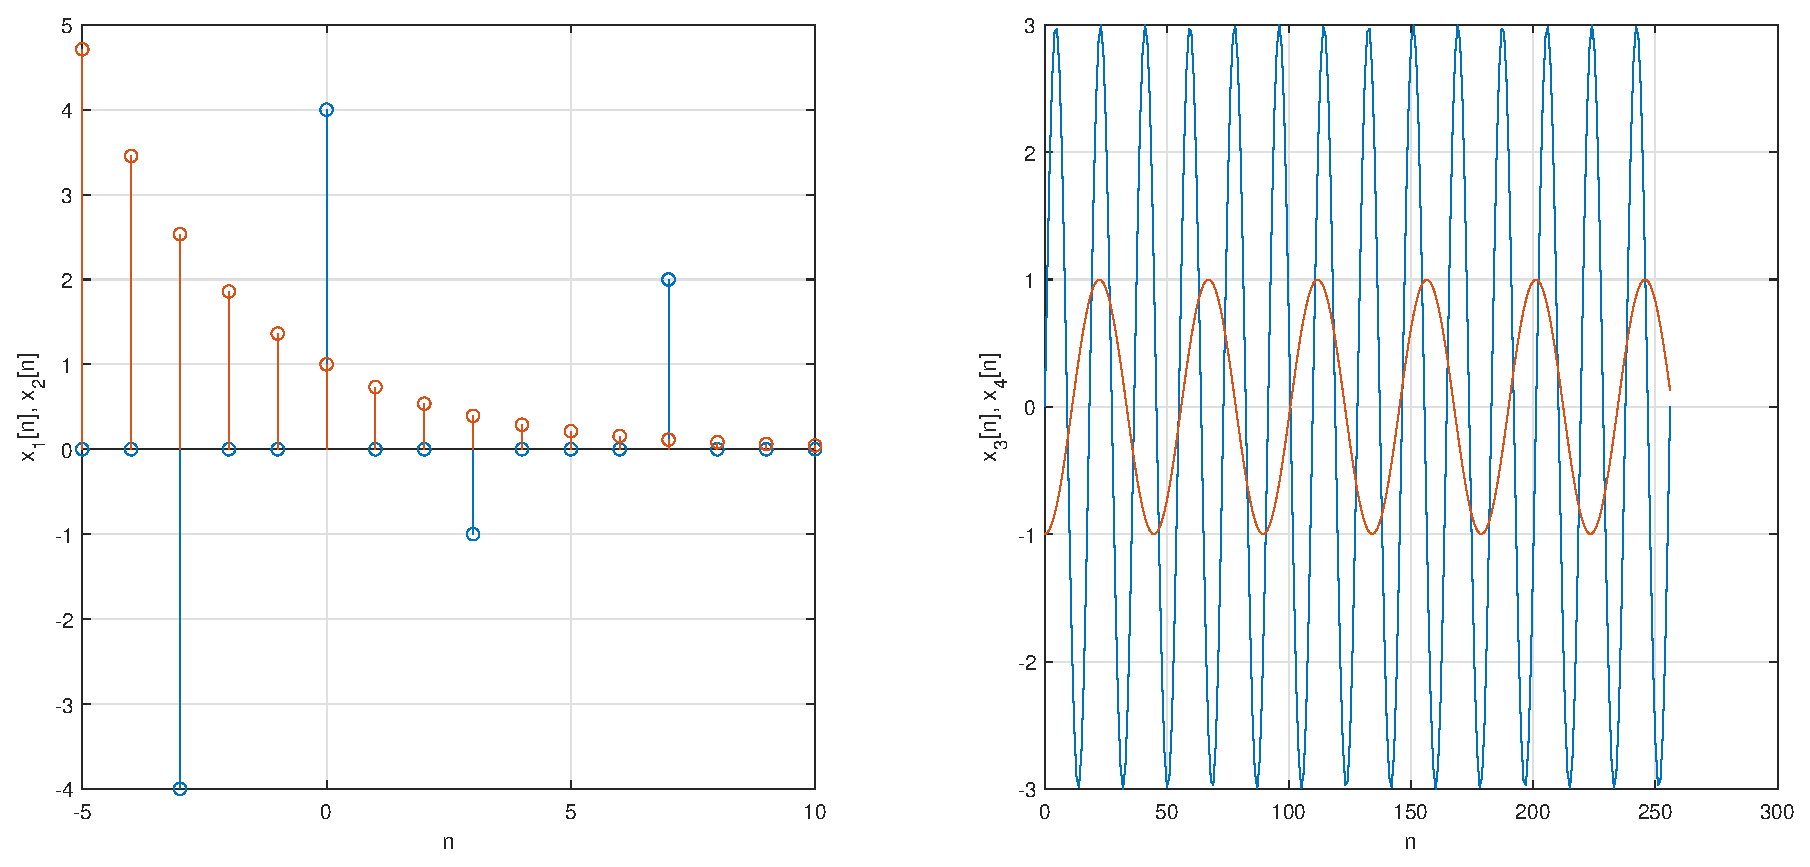
\includegraphics[width=\textwidth]{fig/ex1_1.eps}
            \caption{Discrete time signals $x_1$, $x_2$, $x_3$ and $x_4$. Blue are $x_1$ and $x_3$, orange $x_2$ and $x_4$.}
            \label{fig:ex1_1}
        \end{figure}

        \item The normalized angular frequency of $x_3$ is $\Omega_3 = 2\pi \frac{3.5}{64}$, for $x_4$ it is $\Omega_4 = \frac{9}{64}$.

        \item $x_3$ is periodic with a fundamental period of $128$. $x_4$ is not periodic.

        \item The only periodic signal is $x_3$, the mean power is $4.5$.
        
        \begin{verbatim}
function result = customPower(period)
    result = (1 / length(period)) * sum(power(abs(period), 2));
end
        \end{verbatim}

        \item See f) for energies.
        \begin{verbatim}
function result = energy(signal)
    result = sum(power(abs(signal), 2));
end
        \end{verbatim}

        \item See Table \ref{tab:ex1_1}.
        \begin{table}[htb]
            \centering
            \begin{tabular}{c c c}\toprule
                Signal & Mean power & Energy \\\midrule
                $x_1$ & N/A & 37 \\
                $x_2$ & N/A & 48.0394 \\
                $x_3$ & 4.5 & 1152 \\
                $x_4$ & N/A & 128.9565 \\\bottomrule
            \end{tabular}
            \caption{Table of mean powers and energies.}
            \label{tab:ex1_1}
        \end{table}
    \end{enumerate}
\end{exercise}

\begin{exercise}{Convolution 1}
    \begin{enumerate}
        \item $N_y = N_x + N_h - 1 = 5 + 4 - 1 = 8$
        \item The vector $y$ represents the output signal $y[n]$ where $0 \leq n < 8$.
        \begin{align*}
            y = X h = \begin{bmatrix}
                3  & 0  & 0  & 0 \\
                -1 & 3  & 0  & 0 \\
                2  & -1 & 3  & 0 \\
                0  & 2  & -1 & 3 \\
                1  & 0  & 2  & -1\\
                0  & 1  & 0  & 2 \\
                0  & 0  & 1  & 0 \\
                0  & 0  & 0  & 1
            \end{bmatrix}
            \begin{bmatrix}
                2 \\
                3 \\
                4 \\
                1
            \end{bmatrix}
            =
            \begin{bmatrix}
                6 \\
                -2 + 9 \\
                4 - 3 + 12 \\
                6 - 4 + 3 \\
                2 + 8 - 1 \\
                3 + 2 \\
                4 \\
                1
            \end{bmatrix}
            =
            \begin{bmatrix}
                6 \\
                7 \\
                13 \\
                5 \\
                9 \\
                5 \\
                4 \\
                1
            \end{bmatrix}
        \end{align*}
    \end{enumerate}
\end{exercise}

\begin{exercise}{Convolution 2}
    \begin{enumerate}
        \item $L_y = N_x + N_h - 1 = 50 + 3 - 1 = 52$
        \item \begin{verbatim}
function y = custom_conv(x, h)
    l_x = length(x);
    l_h = length(h);

    l_y = l_x + l_h - 1;

    y = zeros(1, l_y);

    % for every output element...
    for n = 1:l_y
        % (sum index) for every h index...
        for i = 0:l_h-1
            % make sure we don't have any out-of-bounds accesses
            if n - i > 0 && n - i <= l_x
                y(n) = y(n) + h(i + 1) * x(n - i);
            end
        end
    end
end
        \end{verbatim}
        \item See Figure \ref{fig:ex3_1}.
        \begin{figure}[htb]
            \centering
            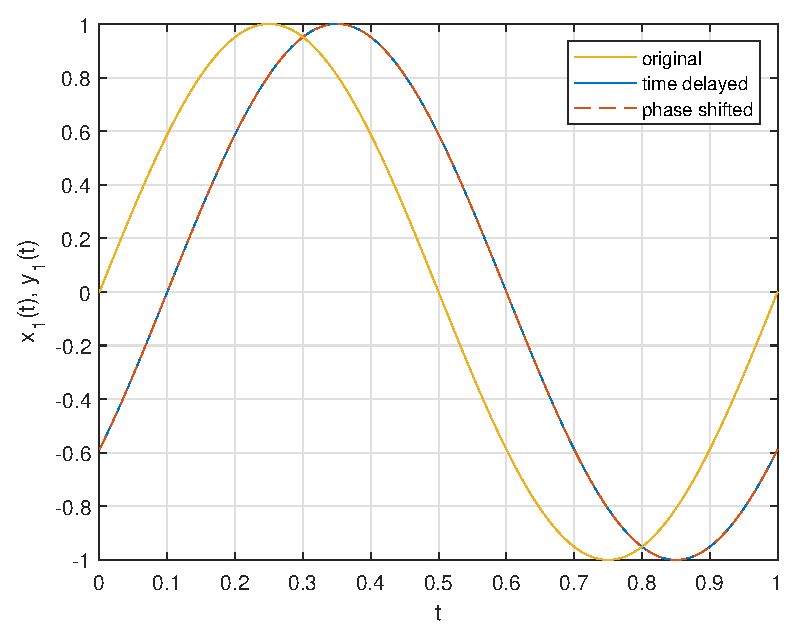
\includegraphics{fig/ex3_1.eps}
            \caption{Plot of $y[n]$.}
            \label{fig:ex3_1}
        \end{figure}
        \item See Figure \ref{fig:ex3_2}
        \begin{figure}[htb]
            \centering
            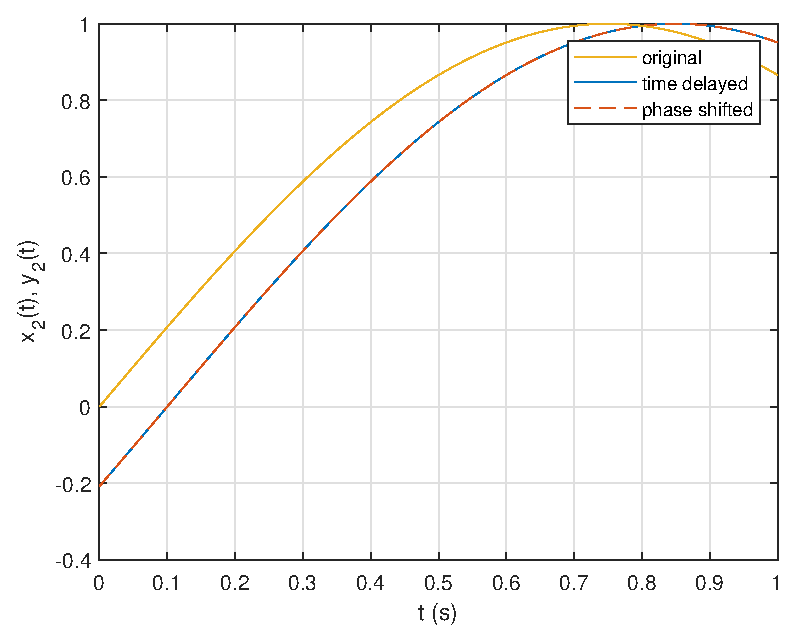
\includegraphics{fig/ex3_2.eps}
            \caption{Plot of $y[n]$ with custom and built-in convolution function.}
            \label{fig:ex3_2}
        \end{figure}
    \end{enumerate}
\end{exercise}

\begin{exercise}{Discrete Time Fourier Transform}
    Note that only $x[n]$ for $-10 \leq n \leq 11$ is relevant, the sequence is 0 for all other $n$.
    \begin{enumerate}
        \item \begin{verbatim}
function X = dtft(x, n, w)
    X = x * exp(-1j * w .* n');
end
        \end{verbatim}

        The core idea is to use element-wise multiplication of $w$ and $n^T$ to produce a matrix like
        \begin{align*}
            \begin{pmatrix}
                w_0n_0 & w_1n_0 & \cdots & w_nn_0 \\
                w_0n_1 & w_1n_1 & \cdots & w_nn_1 \\
                \vdots & \vdots & \ddots & \vdots \\
                w_0n_m & w_1n_m & \cdots & w_nn_m
            \end{pmatrix}
        \end{align*}
        which is then trivially adjusted such that each element $\alpha$ turns into $e^{-j\alpha}$.

        We can then use matrix multiplication of the row vector $x$ with the matrix we just produced to multiply in the relevant $x[n]$s and sum over the columns.
        
        \item See Figure \ref{fig:ex4_1}.
        \begin{figure}[htb]
            \centering
            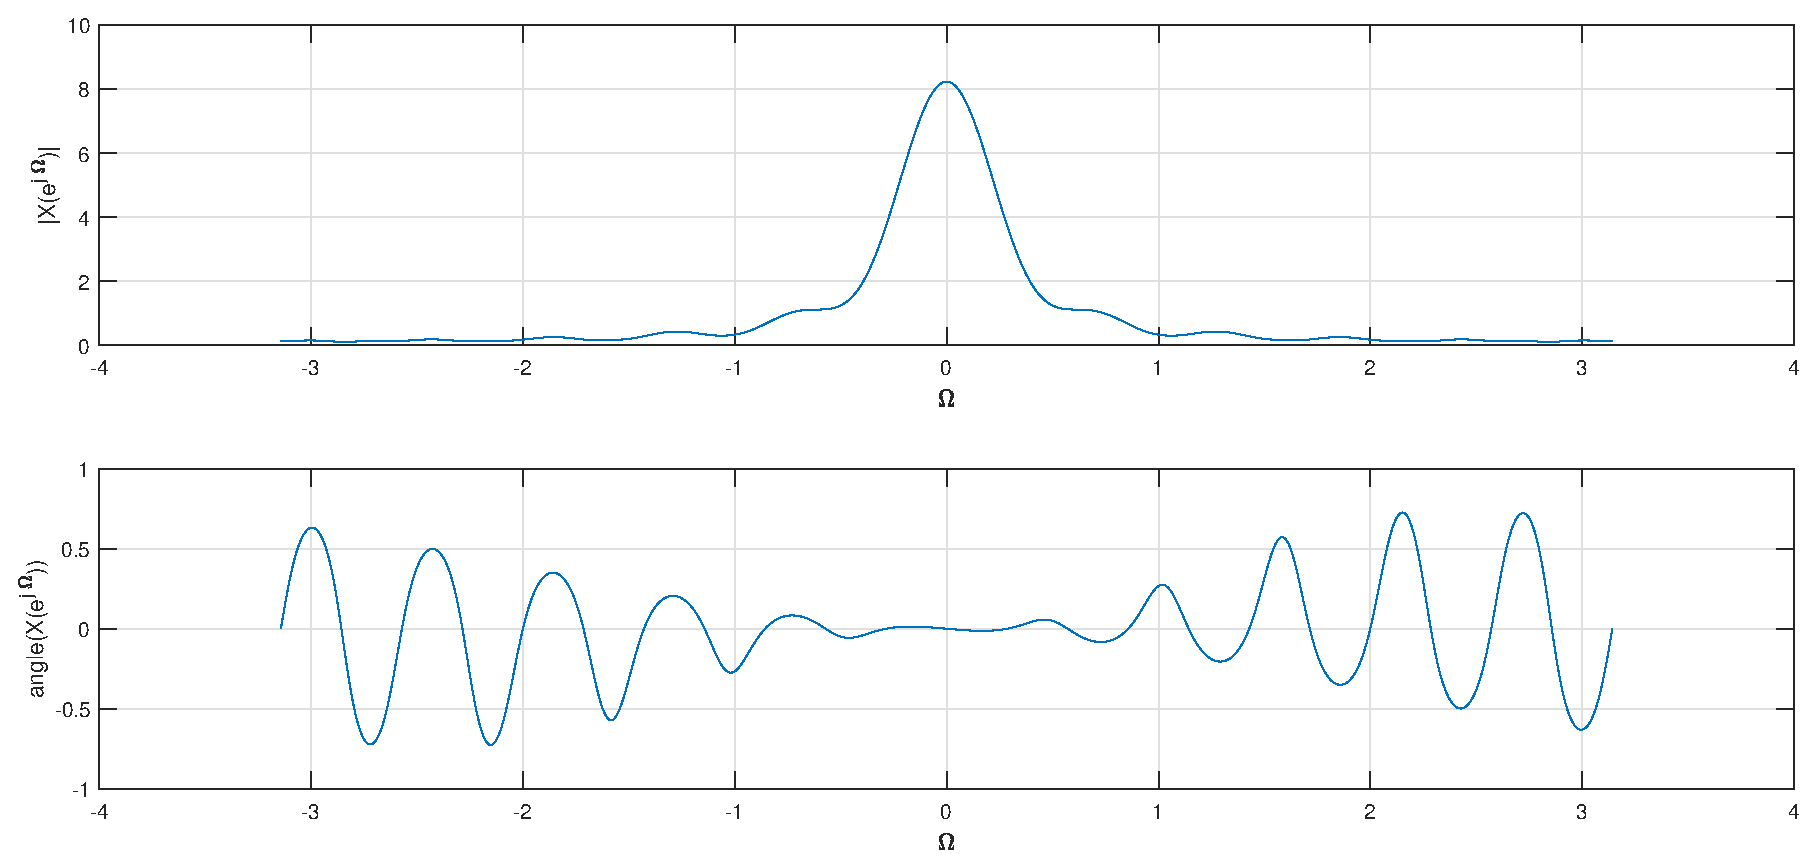
\includegraphics[width=\textwidth]{fig/ex4_1.eps}
            \caption{Magnitude and phase response of $X(e^{j\Omega})$ for $-\pi \leq \Omega \leq \pi$}
            \label{fig:ex4_1}
        \end{figure}

        \item Increasing $\Omega$ shows the periodicity, see Figure \ref{fig:ex4_2}.
        \begin{figure}[htb]
            \centering
            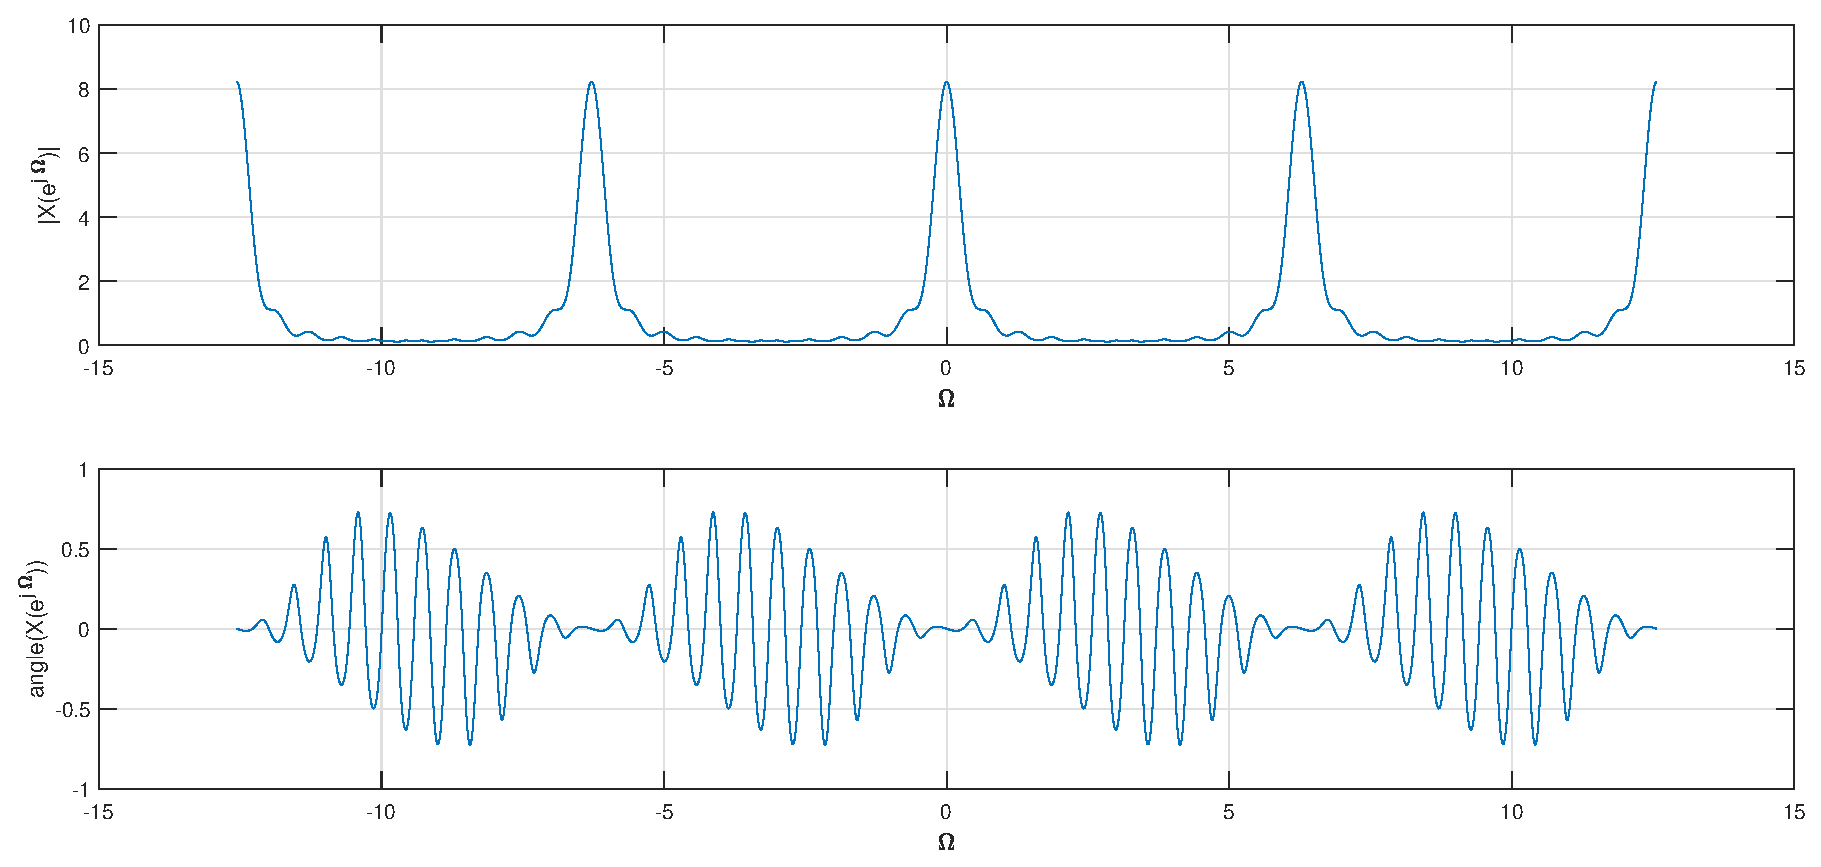
\includegraphics[width=\textwidth]{fig/ex4_2.eps}
            \caption{Magnitude and phase response of $X(e^{j\Omega})$ for $-4\pi \leq \Omega \leq 4\pi$}
            \label{fig:ex4_2}
        \end{figure}
    \end{enumerate}
\end{exercise}

\end{document}
